 \subsection{Cremmer-Gervais $i \mapsto i+1$}
The initial quiver for $\gc_h^{\dagger}(\bg,\GL_4)$ is illustrated in Figure~\ref{f:n=4_CG_i-i+1}.

\begin{figure}[htb]
\begin{center}
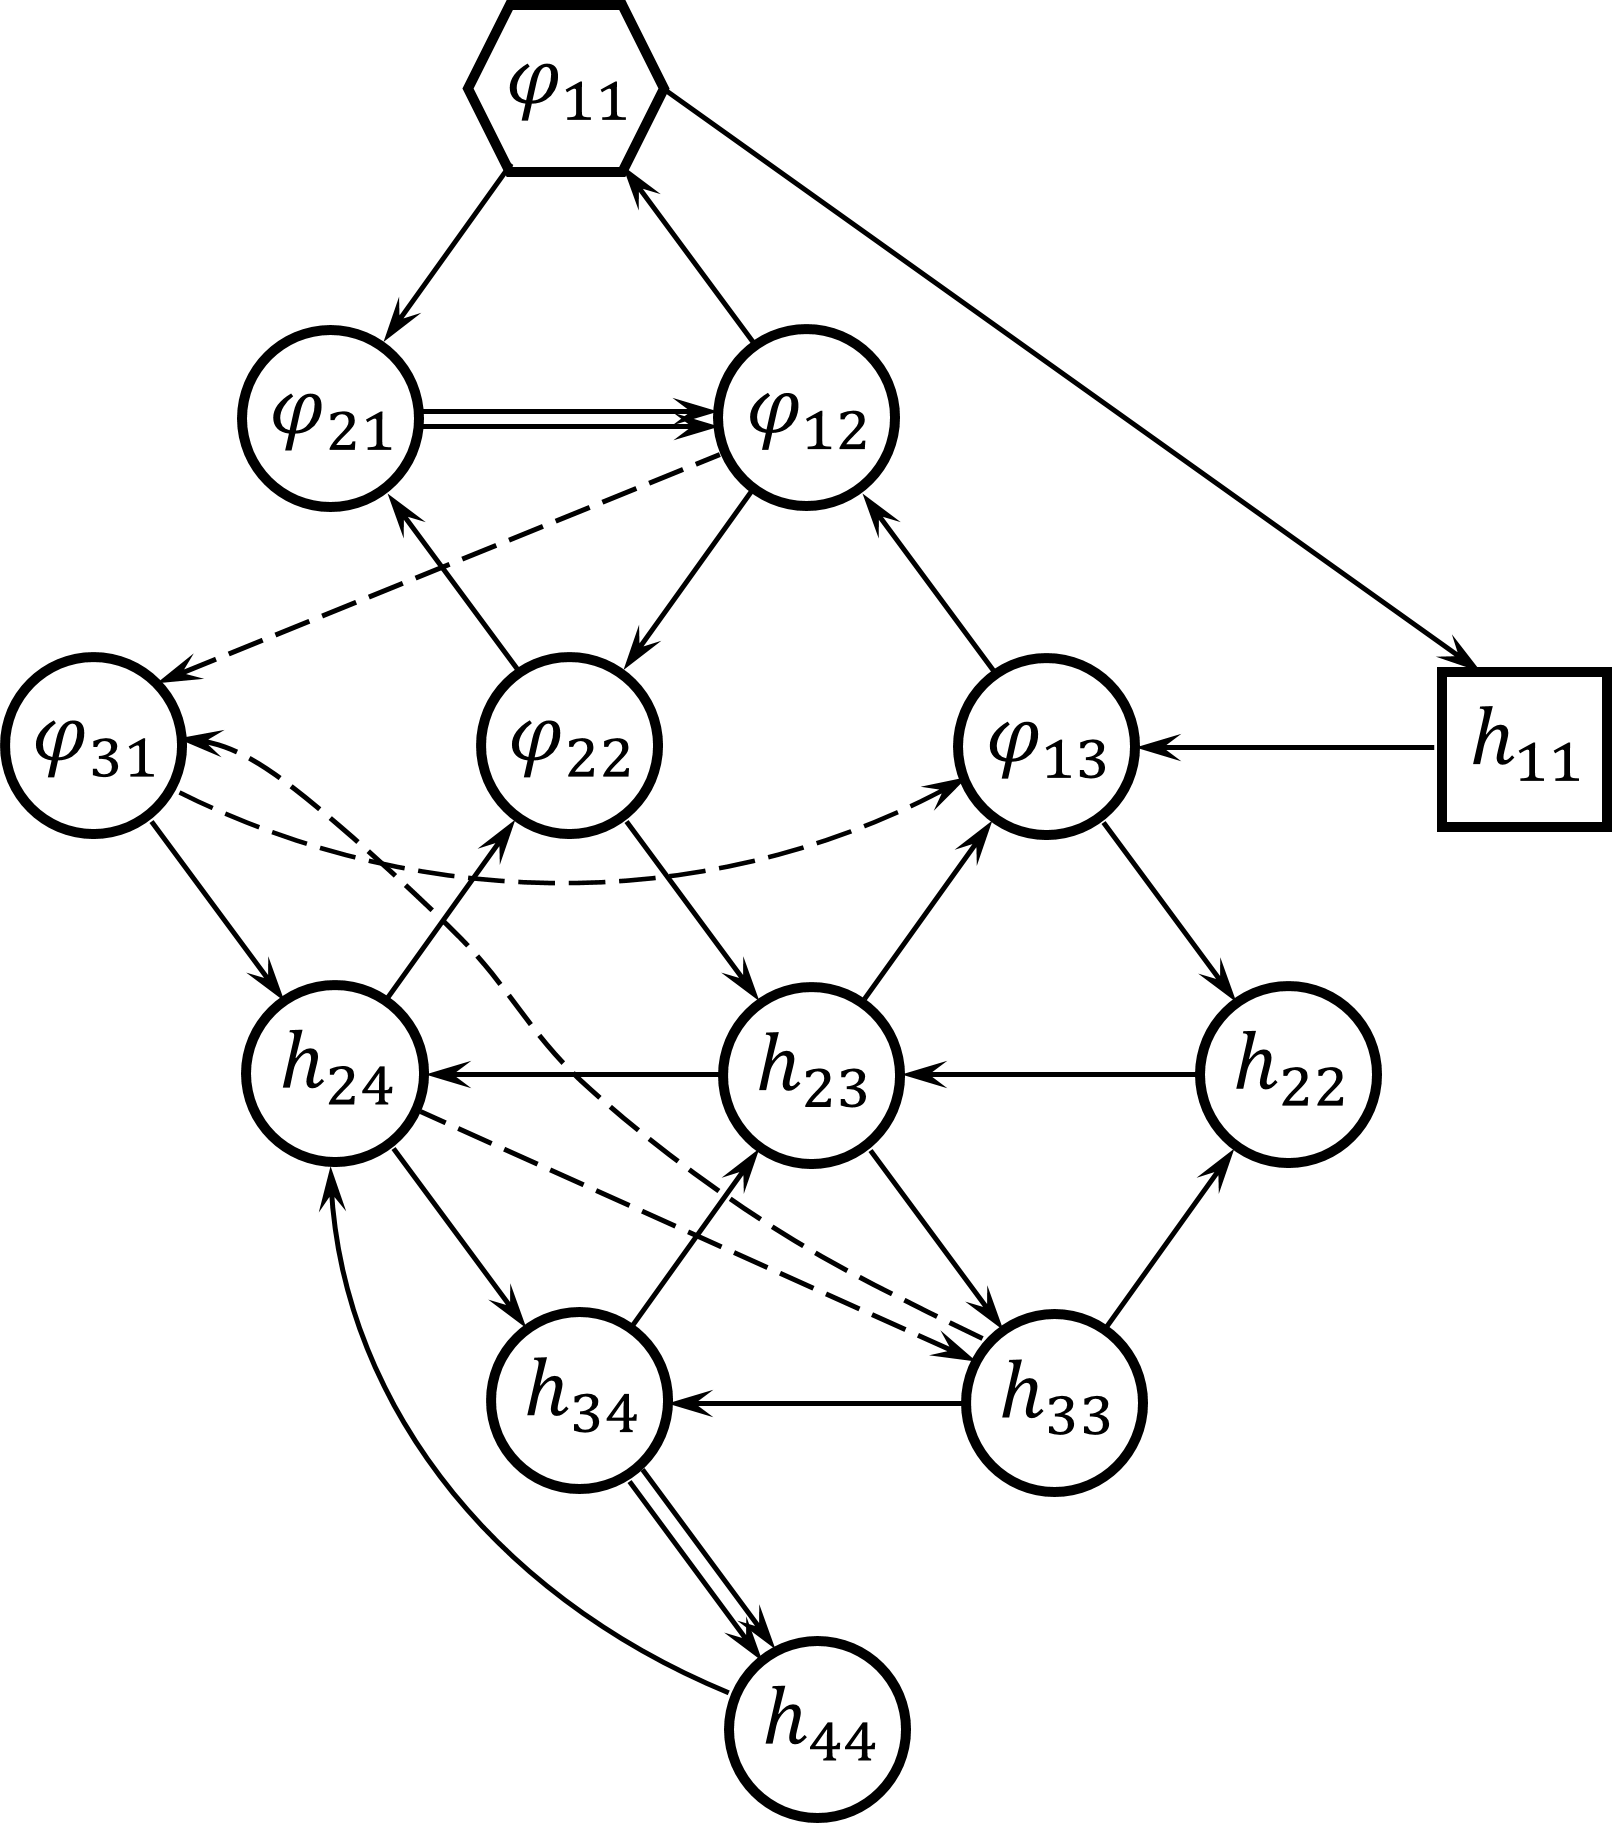
\includegraphics[scale=0.65]{h_convention/h_n=4_CG_i-i+1.png}
\end{center}
\caption{The initial quiver for $\gc^{\dagger}_h(\bg,\GL_4)$ for $\Gamma_1 = \{1,2\}$, $\Gamma_2 = \{2,3\}$, $\gamma:i \mapsto i+1$.}
\label{f:n=4_CG_i-i+1}
\end{figure}
 
 \paragraph{The initial variables.} In the initial extended cluster, all cluster and frozen variables are given as in $\gc_h^{\dagger}(\bg_{\std},\GL_4)$ except for the variables $h_{22}$, $h_{23}$, $h_{24}$, $h_{33}$, $h_{34}$. Let us set
\begin{align}
    &\ell_1(U) := \det U^{[3,4]}_{[3,4]}u_{44} +\det U_{\{2,4\}}^{[3,4]} u_{43}+ \det U^{[3,4]}_{\{1,4\}} u_{42};\\
    &\ell_2(U) := \det U_{[3,4]}^{\{2,4\}}u_{44} +\det U_{\{2,4\}}^{\{2,4\}} u_{43}+ \det U^{\{2,4\}}_{\{1,4\}} u_{42};\\
    &\ell_3(U) := \det U_{[3,4]}^{[2,3]}u_{44} +\det U_{\{2,4\}}^{[2,3]} u_{43}+ \det U^{[2,3]}_{\{1,4\}} u_{42}.
\end{align}
Then the $h$-variables are given by:
\begin{align}
    &h_{24}(U) = u_{24}\cdot \ell_1(U) + u_{14}\ell_2(U), \ \ h_{34}(U) = -u_{34}u_{44} - u_{24}u_{43} - u_{14}u_{42}, \ \ h_{44}(U) = u_{44}; \\
    &h_{23}(U) = \det U^{[3,4]}_{[2,3]}\ell_1(U) + \det U^{[3,4]}_{\{1,3\}}\ell_2(U) + \det U^{[3,4]}_{[1,2]}\ell_3(U), \ \ h_{33}(U) = \ell_1(U);\\
    &h_{22}(U) = \det U^{[2,4]}_{[2,4]}\ell_1(U) + \det U_{\{1\}\cup[3,4]}^{[2,4]}\ell_2(U) + \det U^{[2,4]}_{[1,2]\cup\{4\}}\ell_3(U).
\end{align}

 \paragraph{Birational quasi-isomorphisms.} TBD